\tikzsetnextfilename{fig-cubic-consecutive-2}
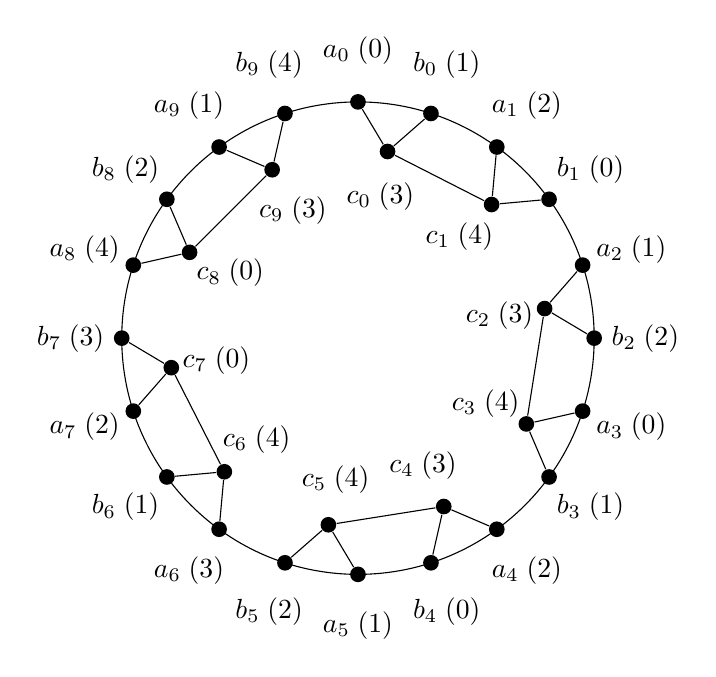
\begin{tikzpicture}[scale=1,
    vertex/.style={circle, fill=black, inner sep=2pt}
]

% Círculo exterior
\draw (0,0) circle (3cm);

% Vértices a_i, b_i
\foreach \i/\name/\col in {
    0/$a_0$/0,  1/$b_0$/1,
    2/$a_1$/2,  3/$b_1$/0,
    4/$a_2$/1,  5/$b_2$/2,
    6/$a_3$/0,  7/$b_3$/1,
    8/$a_4$/2,  9/$b_4$/0,
    10/$a_5$/1, 11/$b_5$/2,
    12/$a_6$/3, 13/$b_6$/1,
    14/$a_7$/2, 15/$b_7$/3,
    16/$a_8$/4, 17/$b_8$/2,
    18/$a_9$/1, 19/$b_9$/4}
{
    \node[vertex] (v\i) at ({90-18*\i}:3) {};
    \node [shift=({90-18*\i}:0.65)] at (v\i) {\name\;(\col)};
}

% Vértices c_i, centrados entre a_i y b_i
\foreach \i/\name/\col in {
    0/$c_0$/3, 1/$c_1$/4,
    2/$c_2$/3, 3/$c_3$/4,
    4/$c_4$/3, 5/$c_5$/4,
    6/$c_6$/4, 7/$c_7$/0,
    8/$c_8$/0, 9/$c_9$/3}
{
    \node[vertex] (c\i) at ({81-36*\i}:2.4) {};
    \node [shift=({81-36*\i}:-0.58)] at (c\i) {\name\;(\col)};
}

% Aristas a_i-c_i y b_i-c_i
\foreach \i in {0,...,9}
{
    \pgfmathtruncatemacro{\a}{2*\i}
    \pgfmathtruncatemacro{\b}{2*\i+1}
    \draw (v\a)--(c\i)--(v\b);
}

% Aristas del matching M
\draw (c0)--(c1);
\draw (c2)--(c3);
\draw (c4)--(c5);
\draw (c6)--(c7);
\draw (c8)--(c9);

\end{tikzpicture}